\chapter{Introduction\label{chap:intro}}

% Cold start
In this thesis, we develop an exact declarative programming based algorithmic approach for finding so-called Pareto-optimal solutions to bi-objective optimization problems encoded in propositional logic.

% What are optimization problems and where do they occur
% Start by telling a story (running example throughout intro)
Optimization problems can be summarized as the task of finding a ``best'' solution out of a collection of feasible ones.
For example, when looking for a new flat to buy, most people will be comparing prices with the aim to find the cheapest flat possible that fulfils their requirements.
Commonly, the notion of ``best'' that is used in optimization is that a solution with lowest associated ``cost'' is considered optimal.
Speaking in the example from above, cost is the price of a flat.
If the collection of possible solutions is discrete (as in this example), we speak of \emph{combinatorial} optimization.

% Real-world problems and hardness
For most problems appearing in the real-world, the set of feasible solutions is too large to represent explicitly.
Instead, the feasible solutions are implicitly represented, often as a set of constraints.
Solving such an implicitly defined optimization problem is typically \NP-hard~\autocite{AroraBarak2009-complexity} and requires non-trivial algorithmic approaches.
Examples of \NP-hard optimization problems can be found in the literature for scheduling~\autocites{DBLP:conf/cp/Stojadinovic14,DBLP:conf/cpaior/BofillGSV15,DBLP:journals/ior/Solomon87,DBLP:journals/candie/AkyolB07}, supply chain optimization~\autocite{DBLP:journals/cce/Papageorgiou09}, air traffic management~\autocites{DBLP:journals/ior/BertsimasLO11,RichardsHow2002Aircrafttrajectoryplanning}, clustering~\autocite{DBLP:journals/ai/DaoDV17,DBLP:conf/sdm/DavidsonRS10}, learning optimal classifiers~\autocites{DBLP:conf/cp/MaliotovM18,DBLP:conf/ijcai/NarodytskaIPM18,DBLP:conf/ijcai/Hu0HH20,DBLP:conf/cp/YuISB20,DBLP:conf/aaai/DemirovicS21,DBLP:conf/cp/ShatiCM21,DBLP:conf/cade/IgnatievPNM18}, and much more.

% Approaches to solving optimization
Different approaches for finding optimal solutions to \NP-hard problems have been proposed.
In local search~\autocite{DBLP:books/daglib/0017492} a candidate solution is iteratively modified to find a better and hopefully optimal solution.
Evolutionary algorithms~\autocites{DBLP:books/daglib/0087893,DBLP:journals/jgo/StornP97} maintain a set of solutions that develops over time, where only the best candidates are kept.
In declarative programming based algorithms~\autocite{handbook2-maxsat,ChenEtAl2010-intro,DBLP:reference/fai/2} the problem is encoded as constraints formulated in a declarative programming language.
A solution is then found with a solving algorithm for the used declarative programming language.
In addition to these generally applicable approaches, there are problem specific algorithms (e.g.,~\autocite{DBLP:conf/aaai/DemirovicS21,DBLP:conf/kdd/NijssenF07,DBLP:conf/nips/HuRS19}).
One other attribute on which the optimization approaches differ is whether they are exact or inexact.
Given enough resources, an exact algorithm is guaranteed to find \emph{the best} solution, while inexact algorithms will return \emph{a good} solution within given resource constraints.

% Solving pipeline for declarative approaches
The exact declarative programming approach solves optimization problems by first encoding the original problem into a set of constraints formulated in an encoding language.
An encoding is hereby a mapping of each instance of the original problem to a set of constraints in the declarative language, where each optimal solution to the encoded instance corresponds to an optimal solution to the original instance.
Having encoded the problem, an algorithm for finding an optimal solution to the encoded problem---called a solver---is invoked on the encoded instance to find a solution with the lowest cost.
As a last step, this found solution to the encoded instance is mapped back to the original problem space.
This solving pipeline for the declarative approach is illustrated in \cref{fig:solving-pipeline}.

\begin{figure}
  \centering
  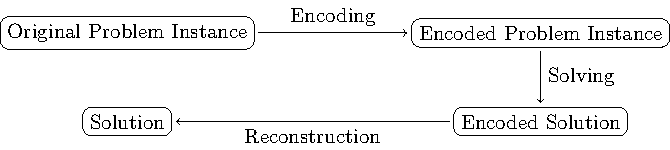
\includegraphics{solving-pipeline.pdf}
  \caption{The solving pipeline of the declarative approach to optimization.}\label{fig:solving-pipeline}
\end{figure}

% Advantages of the declarative approach and languages
The advantage of the declarative approach is that it is generally applicable to every problem for which an encoding exists.
When solving an optimization problem with the declarative approach, the challenge lies in choosing the encoding language that allows for a natural encoding and finding such an encoding, not in designing an algorithm.
Arguably, the most classical language for modelling \NP-hard optimization problems is that of mixed integer linear programming (MILP)~\autocites{ChenEtAl2010-intro,KorteVygen2018-5}.
It might come as a surprise that the encoding language of propositional logic---which is very limited in expressiveness---has seen a stark increase in usage as well.
However, recent research has achieved good results by using maximum satisfiability (MaxSAT)~\autocite{handbook2-maxsat}, the optimization variant of propositional satisfiability (SAT)~\autocite{handbook2-sat}.
Both, MILP and MaxSAT, are \NP-hard encoding languages;
typically, the same holds for other used languages as well.
This allows for the encoding to be polynomial in size for \NP-hard optimization problems.
Given an existing encoding, the computationally hard step in the declarative solving pipeline therefore is the call to the solver, having exponential runtime in the worst case.
However, examples of solving algorithms that exibit significantly better than worst-case performance on real-world instances are branch-and-cut algorithms for mixed integer linear programming~\autocite{ChenEtAl2010-branch-and-cut}, and MaxSAT solving algorithms~\autocite{handbook2-maxsat} based on conflict driven clause learning solvers for propositional satisfiability~\autocite{handbook2-cdcl}.

% Reveal conflicting second objective
It should be noticed that a clear majority of declarative optimization approaches, including MILP and MaxSAT, work under the assumptions that we are dealing with problems which intrinsically have a single objective to optimize.
However, this is not always the case.
Coming back to the flat search example, we notice that some requirements, like the number of rooms, might be easy to specify, but consider the distance of ones daily commute.
Rather than setting a fixed threshold as ``maximum $d$ kilometres distance'', what we might actually want to do is minimize this distance at the same time as the cost of the flat.
Now there are two objectives to take into account regarding what constitutes a ``best'' solution.
Two objectives give rise to \emph{bi-objective} optimization.

% Applications of bi-objective optimization in literature
Bi-objective optimization problems arise naturally for various real-world settings.
For example, when learning interpretable classifiers~\autocites{DBLP:conf/ijcai/Ignatiev0NS21,DBLP:conf/cp/MaliotovM18,DBLP:conf/ijcai/NarodytskaIPM18,DBLP:conf/ijcai/Hu0HH20,DBLP:journals/corr/abs-2010-09919,DBLP:conf/cp/YuISB20,DBLP:conf/aaai/Ignatiev0S021,DBLP:conf/cade/IgnatievPNM18}, the objectives ``interpretability'' and ``classification error'' are in conflict because a more complex and therefore less interpretable classifier is typically more accurate.
As another example, a bi-objective optimization problem arises when wanting to create a portfolio of solvers that together solve a set of benchmarks as fast as possible while also containing as few solvers as possible~\autocite{DBLP:conf/cp/JanotaMSM21}.
There are also bi-objective optimization problems in network routing with the objectives load balancing and latency~\autocite{SilverioEtAl2022biobjectiveoptimization}.
In supply chain optimization, in addition to the economic objective, environmental aspects can be taken into consideration as a second objective~\autocites{DBLP:journals/cce/Pinto-VarelaBN11,DBLP:journals/candie/TautenhainBN19}.
In this thesis, we apply the declarative approach to find exact solutions to such bi-objective optimization problems.

% Conflicting objectives and why there might be no single optimal solution
A crucial difference between single-objective and bi-objective optimization is that there is no single notion of optimality for two or more objectives.
Whereas for a single objective function, there is a clear minimum (or maximum) and objective values can be unambiguously compared, this becomes less defined for the bi-objective case:
in the flat search example, consider a flat A with a cost of 300\,000 \texteuro{} and 1-kilometre daily commute and compare it to another flat B that costs 240\,000 \texteuro{} and has a 3-kilometre daily commute.
It is not immediately clear which one of these options is better, and the choice would depend on ones personal preference over the two objectives.
This becomes especially difficult if there is no such preference.
Typically, a situation like that occurs when two of the objectives considered are in conflict, as the price of a flat and the corresponding daily commute might be if the commute is towards the city centre and flats in the city centre are more expensive.

% Pareto optimality
% Point out different nomenclature
As common in other work, in the context of this thesis, the notion of optimality for bi-objective optimization is that of \emph{Pareto optimality} (also called \emph{efficiency} in other contexts, e.g.,~\autocite{DBLP:journals/siamjo/SantisENR20})~\autocite{Ehrgott2005-2}.
Intuitively, under Pareto optimality a solution is considered optimal if no solutions that improve some objective without worsening the other exist.
As an example, this definition considers the two flats A and B from earlier both equally optimal.
Under Pareto optimality, the task of solving a bi-objective optimization problem can mean multiple things:
finding a single Pareto-optimal solution, finding a representative solution for each Pareto point (i.e., tuple of Pareto-optimal objective values, also called non-dominated point in literature~\autocite{Ehrgott2005-2}), or finding all Pareto-optimal solutions.
Most approaches~\autocite{DBLP:conf/cp/SohBTB17,DBLP:conf/cp/JanotaMSM21,DBLP:conf/ijcai/Terra-NevesLM18a} to solving multi-objective optimization under Pareto optimality appear to focus on the second task where a single solution per Pareto point is computed.
The last task goes one step further and enumerates the full Pareto front (i.e., all Pareto-optimal solutions), even if multiple of the solutions might lead to the same objective values.
All three of these tasks can be solved by the algorithmic approach presented in this thesis.

% Bi-objective vs multi-objective
% Why bi-objective is interesting/enough
Beyond the bi-objective setting, multi-objective optimization problems with an arbitrary number of objectives may also be considered.
In that situation, the handle on what the multiple objective values of an optimal solution actually mean can quickly become hard to grasp.
The human mind can only visualize three dimensions, meaning a Pareto front over four objectives is already entirely abstract while even a three-dimensional one is hard to visualize.
Two objectives, form a good trade-off between gaining meaningful information from the second objective over just using a single one, being able to intuitively visualize the Pareto front, and not resulting in too many Pareto-optimal solutions.
Furthermore, additional objectives can still be added as threshold constraints.

% Contributions
% Algorithm: single SAT solver; builds on MaxSAT; single vs all
The main contribution of this work is the \algname{} algorithm, a MaxSAT-based bi-objective optimization approach.
\algname{} follows the lexicographic method~\autocite{survey}, which works by minimizing the objective which we call increasing first and afterwards minimizing the decreasing objective under the constraint that the increasing one cannot get worse.
Once the first Pareto point has been found, the search continues by minimizing the increasing objective again, but under the constraint that the decreasing objective should be smaller than before.
Note the difference between this lexicographic \emph{method} compared to lexicographic \emph{optimization}~\autocite{DBLP:conf/ijcai/ArgelichLS09,DBLP:journals/amai/Marques-SilvaAGL11} to which SAT-based approaches have been proposed earlier.
Lexicographic optimization only considers the first Pareto point, found by the lexicographic method, optimal.

% Variants
\algname{} builds on advances in MaxSAT solving, allowing for variants based on different solution-improving~\autocites{handbook2-maxsat,DBLP:journals/jsat/BerreP10,DBLP:journals/jsat/EenS06} and core-guided~\autocites{DBLP:journals/corr/abs-0712-1097,DBLP:conf/sat/AnsoteguiBL09,DBLP:conf/cp/MorgadoDM14,DBLP:journals/jsat/IgnatievMM19} algorithms.
We propose five different variants of \algname{} that differ in how the minimization of the increasing objective is done.
The first four building on the SAT-UNSAT~\autocite{DBLP:journals/jsat/BerreP10}, UNSAT-SAT~\autocite{DBLP:conf/sat/FuM06}, MSU3~\autocite{DBLP:journals/corr/abs-0712-1097} and OLL~\autocite{DBLP:conf/cp/MorgadoDM14} MaxSAT algorithms, modifying them mainly in the fact that a bound on the decreasing objective needs be enforced during optimization.
The fifth variant is a hybrid switching from the MSU3- to the SAT-UNSAT-based variant during the search, aiming to combine the advantages of the two approaches.
In addition to five variants of \algname{}, we also propose multiple refinements for improving its performance:
lazily building the cardinality constraints for both objectives to reduce the number of clauses in the solver, blocking dominated solutions to prune the search space, more efficient domain-specific blocking clauses, bound hardening to enable the solver to learn more information and other refinements known from core-guided MaxSAT solving.
\algname{} allows for solving all three tasks for bi-objective optimization:
finding a single Pareto-optimal solution, one representative solution for each Pareto point or enumerating all Pareto-optimal solutions.

% Evaluation: study efficiency of different MaxSAT algorithms
We provide an open-source implementation of all five variants of \algname{} ({\small\url{https://bitbucket.org/coreo-group/bioptsat/}}) and empirically evaluate its performance on two benchmark domains:
learning interpretable decision rules from binary data~\autocite{DBLP:conf/cp/MaliotovM18} (as a generalization of settings for which MaxSAT-based single-objective solutions have been proposed previously) and bi-objective set covering.
In the experiments, we compare \algname{} to three SAT-based competitors:
enumeration of $P$-minimal solutions~\autocite{DBLP:conf/cp/SohBTB17}, ParetoMCS enumeration~\autocite{DBLP:conf/ijcai/Terra-NevesLM18a} and Seesaw~\autocite{DBLP:conf/cp/JanotaMSM21}.
We find that \algname{} outperformed these competitors in all studied cases.
As an additional result of this evaluation, we determine which variant of \algname{} is the best-performing overall.
Furthermore, for the best-performing variant, we study the effects of the proposed refinements to determine their effectiveness.

% Acknowledging the paper
Results presented in this thesis have been published in the proceedings of the 25th International Conference on Theory and Applications of Satisfiability Testing (SAT 2022)~\autocite{JabsEtAl2022MaxSATBasedBi}.
In this thesis, we extend on the evaluation and give a more in depth description of the preliminaries and the algorithm itself, compared to~\autocite{JabsEtAl2022MaxSATBasedBi}.

% Signposting for chapters
This thesis is structured as follows:
An overview of propositional satisfiability and maximum satisfiability, highlighting the important preliminaries needed to understand the proposed algorithm, is given in \cref{chap:satisfiability}.
In \cref{chap:biobjective-optimization}, we introduce bi-objective optimization, defining the problem and surveying some existing approaches, based on SAT and other declarative paradigms, as well as probabilistic and meta-heuristic approaches.
After that, in \cref{chap:approach}, \algname{}---including five variants and some refinements---is proposed.
Finally, in \cref{chap:experiments} we outline the experiments and results, and conclude the thesis in \cref{chap:conclusion}.